\fancyhead[C]{\textit{Solutions}}

\section{Solutions to Section 1}

\subsection{Activity 1}
	\begin{table}[!h]
		\centering
		\begin{tabular}{c@{\hspace{2.5em}}cp{0.75\textwidth}}
			true & false & \\
			\specialrule{\lightrulewidth}{0.25em}{1.25em}
			\bubble & \dbubble & If a \(m \times n\) matrix \(A\) has \emph{no} zero entry, then the matrix has a pivot in every column. \\[0.75em]
			\bubble & \dbubble & A pivot in every row of an augmented matrix of a system of linear equation implies that the system is consistent.\\[0.75em]
			\dbubble & \bubble & If a \(2 \times 7\) coefficient matrix \(A\) that corresponds to the matrix equation \(A\vec{x} = \vec{b}\) has 2 pivots, 
						        then the corresponding system is consistent for any \(\vec{b} \in \mathbb{R}^2\). \\[0.75em]
			\bubble & \dbubble & If a system of linear equations contains free variables, then there exists an infinite number of solutions. \\[0.75em]
			\dbubble & \bubble & The RREF of a matrix is unique. \\[0.75em]
			\bubble & \dbubble & If a row of an augmented matrix corresponding to a system of linear equations is 
						      \(\begin{bmatrix}0 & 0 & 0 & 2 & | & 0\end{bmatrix}\) then the corresponding system is inconsistent. \\[0.75em]
			\bottomrule
		\end{tabular}
	\end{table}

\section{Solutions to Section 2}
\subsection{Activity 2}
\begin{enumerate}
	\item Any line that passes through the origin. Examples:
	\begin{figure}[!h]	
		\centering
		\begin{minipage}{0.33\textwidth}
		\centering
		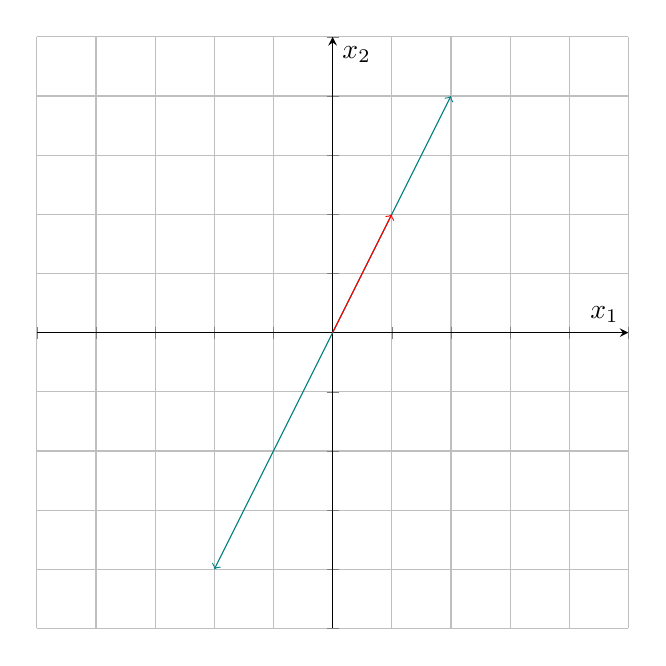
\begin{tikzpicture}
		\begin{axis}[
			height=0.75\textwidth,
			width=0.75\textwidth,
			axis lines = middle,
			xmin=-5, xmax=5, ymin=-5, ymax=5,
			xtick distance=1, ytick distance=1,
			xticklabels={}, yticklabels={,,},
			xlabel=\(x_1\), ylabel=\(x_2\),
			grid=major
		]
		\addplot[<->, color=teal, domain=-2:2, ] {2*x};
		\addplot[->, color=red, domain=0:1]{2*x};
		\end{axis}
	\end{tikzpicture}
	\caption{\(\vspan\left\{\begin{bmatrix}1 \\ 2\end{bmatrix}\right\}\)}
	\end{minipage}\hfill
		\begin{minipage}{0.33\textwidth}
		\centering
		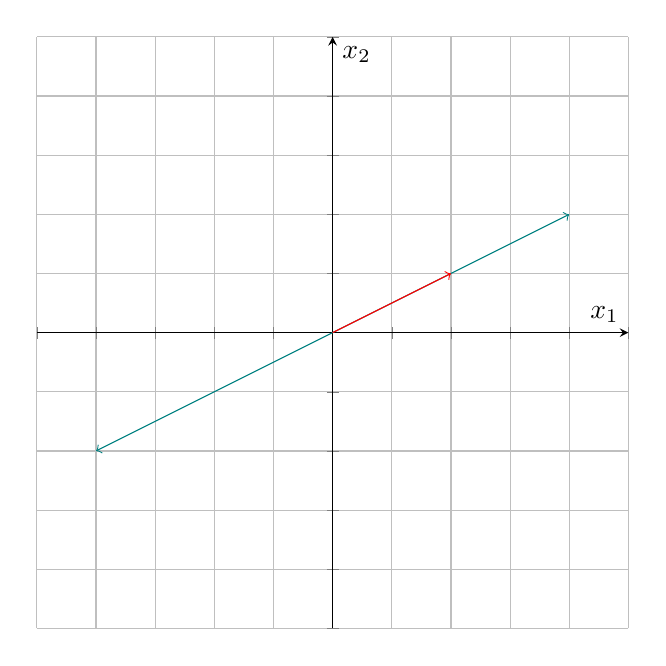
\begin{tikzpicture}
		\begin{axis}[
			height=0.75\textwidth,
			width=0.75\textwidth,
			axis lines = middle,
			xmin=-5, xmax=5, ymin=-5, ymax=5,
			xtick distance=1, ytick distance=1,
			xticklabels={}, yticklabels={,,},
			xlabel=\(x_1\), ylabel=\(x_2\),
			grid=major
		]
		\addplot[<->, color=teal, domain=-4:4, ] {0.5*x};
		\addplot[->, color=red, domain=0:2, ] {0.5*x};
		\end{axis}
	\end{tikzpicture}
	\caption{\(\vspan\left\{\begin{bmatrix}2 \\ 1\end{bmatrix}\right\}\)}
	\end{minipage}\hfill
	\end{figure}

\item Any set of two vectors that are in the span of each other. Examples:
	\begin{figure}[!h]	
		\centering
		\begin{minipage}{0.333\textwidth}
		\centering
		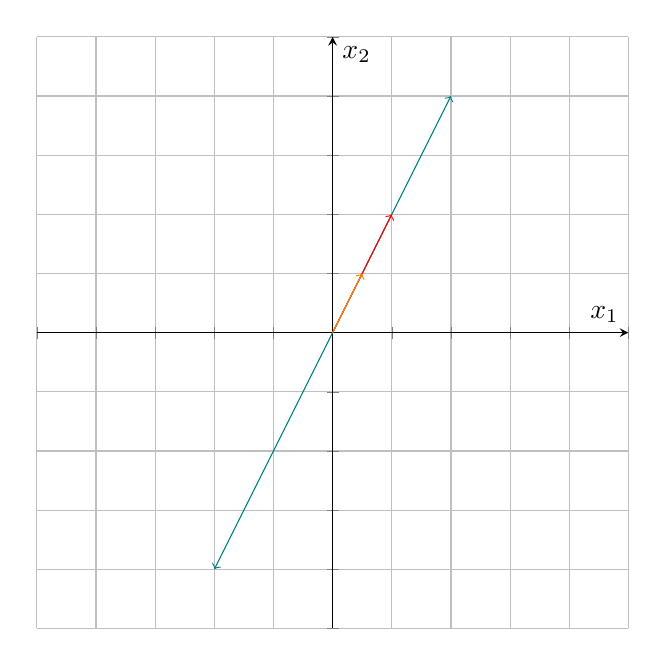
\begin{tikzpicture}
		\begin{axis}[
			height=0.75\textwidth,
			width=0.75\textwidth,
			axis lines = middle,
			xmin=-5, xmax=5, ymin=-5, ymax=5,
			xtick distance=1, ytick distance=1,
			xticklabels={}, yticklabels={,,},
			xlabel=\(x_1\), ylabel=\(x_2\),
			grid=major
		]
		\addplot[<->, color=teal, domain=-2:2] {2*x};
		\addplot[->, color=red, domain=0:1]{2*x};
		\addplot[->, color=orange, domain=0:0.5]{2*x};
		\end{axis}
	\end{tikzpicture}
	\caption{\(\vspan\left\{\begin{bmatrix}1 \\ 2\end{bmatrix}, \begin{bmatrix}0.5 \\ 1\end{bmatrix}\right\}\)}
	\end{minipage}\hfill
		\begin{minipage}{0.33\textwidth}
		\centering
		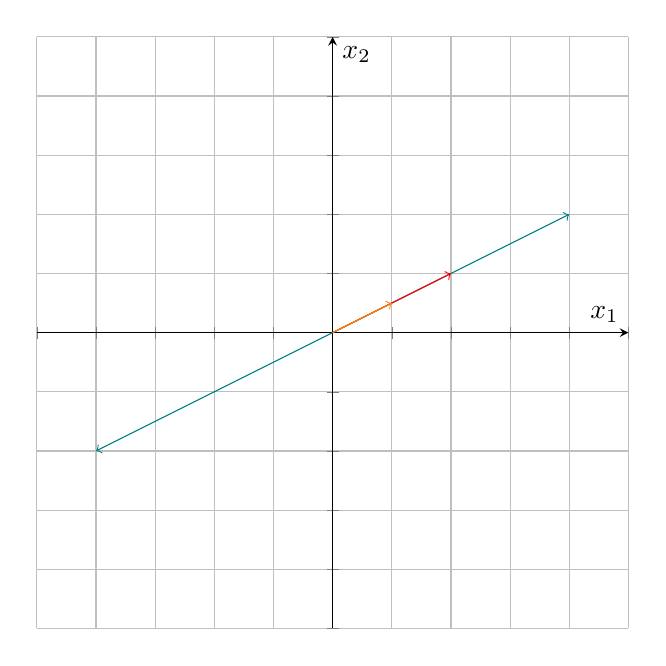
\begin{tikzpicture}
		\begin{axis}[
			height=0.75\textwidth,
			width=0.75\textwidth,
			axis lines = middle,
			xmin=-5, xmax=5, ymin=-5, ymax=5,
			xtick distance=1, ytick distance=1,
			xticklabels={}, yticklabels={,,},
			xlabel=\(x_1\), ylabel=\(x_2\),
			grid=major
		]
		\addplot[<->, color=teal, domain=-4:4, ] {0.5*x};
		\addplot[->, color=red, domain=0:2, ] {0.5*x};
		\addplot[->, color=orange, domain=0:1, ] {0.5*x};
		\end{axis}
	\end{tikzpicture}
	\caption{\(\vspan\left\{\begin{bmatrix}2 \\ 1\end{bmatrix}, \begin{bmatrix}1 \\ 0.5\end{bmatrix}\right\}\)}
	\end{minipage}\hfill
	\end{figure}
\item Most of the time, any three random vectors will work. Examples:
	\begin{figure}[!h]
		\centering
		\begin{minipage}{0.5\textwidth}
			\centering
			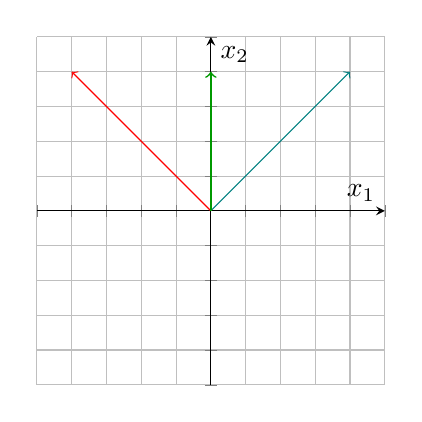
\begin{tikzpicture}
				\begin{axis}[
					height=6cm,
					width=6cm,
					axis lines = middle,
					xmin=-5, xmax=5, ymin=-5, ymax=5,
					xtick distance=1, ytick distance=1,
					xticklabels={}, yticklabels={,,},
					xlabel=\(x_1\), ylabel=\(x_2\),
					grid=major
				]
				\addplot[->, color=teal, domain=0:4]{x};
				\addplot[<-, color=red, domain=-4:0]{-x};
				\draw[->, semithick, color=green!60!black] (axis cs: 0, 0) -- (axis cs: 0, 4);		
				\end{axis}
			\end{tikzpicture}
			\caption{\(\left\{\begin{bmatrix}4 \\ 4\end{bmatrix}, \begin{bmatrix}-4 \\ 4\end{bmatrix}, \begin{bmatrix}0 \\ 4\end{bmatrix}\right\}\)}
		\end{minipage}\hfill
		\begin{minipage}{0.5\textwidth}
			\centering
			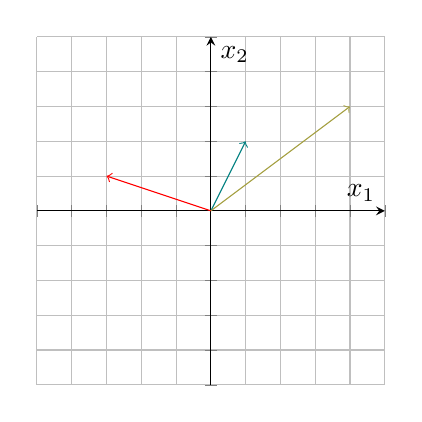
\begin{tikzpicture}
				\begin{axis}[
					height=6cm,
					width=6cm,
					axis lines = middle,
					xmin=-5, xmax=5, ymin=-5, ymax=5,
					xtick distance=1, ytick distance=1,
					xticklabels={}, yticklabels={},
					xlabel=\(x_1\), ylabel=\(x_2\),
					grid=major
				]
				\draw[->, color=teal] (axis cs: 0, 0) -- (axis cs: 1, 2);
				\draw[->, color=red] (axis cs: 0, 0) -- (axis cs: -3, 1);
				\draw[->, color=yellow!60!black] (axis cs: 0, 0) -- (axis cs: 4, 3); 
				\end{axis}
			\end{tikzpicture}
			\caption{\(\left\{\begin{bmatrix}1 \\ 2\end{bmatrix}, \begin{bmatrix}-3 \\ 1\end{bmatrix}, \begin{bmatrix}4 \\ 3\end{bmatrix}\right\}\)}
		\end{minipage}
	\end{figure}
\end{enumerate}

\subsection{Activity 3}
\begin{enumerate}
	\item Yes. To see that, notice that every linear combination of the vectors in the set \(\{2\vec{v}_1 + \vec{v}_2, \vec{v}_2\}\) is a linear combination
		of \(\vec{v}_1\) and \(\vec{v}_2\). Going the other way around, every linear combination of \(\vec{v}_1, \vec{v}_2\) could be shown to be a linear
		combination of \(\{2\vec{v}_1 + \vec{v}_2, \vec{v}_2\}\). To see that, we start with 
			\begin{equation} \label{eq:eq1}
				c_1\vec{v}_1 + c_2\vec{v}_2.
			\end{equation}
		Then, we can set \(c_1 = 2a\) for some real number \(a\), and \(c_2 = a + b\) for some real number \(b\). The main idea is that for each choice of 
		\(c_1, c_2\) we can find the corresponding \(a, b\) such that Equation~\ref{eq:eq1} becomes a linear combination of \(2\vec{v}_1 + \vec{v}_2\) and 
		\(\vec{v}_2\). To show this, note that the system
		\[\left\{\begin{aligned}
			 c_1 &= 2a \\
			 c_2 &= a + b
		\end{aligned}\right.\]
		is \emph{always} consistent. Solving the system in terms for \(a, b\), we find that \(a = \frac{c_1}{2}\) and \(b = c_2 - \frac{c_1}{2}.\) 
		Summarizing our argument, we get 
		\[c_1\vec{v}_1 + c_2\vec{v}_2 = 2a\vec{v}_1 + (a + b)\vec{v}_2 = a (2\vec{v}_1 + \vec{v}_2) + b\vec{v}_2.\] 
		Of course, the reason we can confidently assign \(c_1, c_2\) to combinations of \(a, b\) is because we know that the system above is always 
		consistent.

	\item No. Not always. Look at the sketch you made above!
\end{enumerate}

\subsection{Activity 4}
\begin{enumerate}
	\item If \(\vec{v} \in \vspan \{\vec{b}_1, \vec{b}_2\}\), then there must exist real scalars \(c_1, c_2\) such that 
		\[\vec{v} = c_1\vec{b}_1 + c_2\vec{b}_2 \iff \begin{bmatrix}3 & 1 \\ 6 & 3 \\ 2 & 7\end{bmatrix}\begin{bmatrix}c_1 \\ c_2\end{bmatrix} 
	   	= \begin{bmatrix}1 \\ 5 \\ 8\end{bmatrix}.\]
		Oh, this is the matrix equation \(A\vec{x} = \vec{v}\) that corresponds to a system of linear equation! We know how to solve those!
		If you row reduce, you'll realize that the system is inconsistent. You can then state \(\vec{v} \not\in \vspan\{\vec{b}_1, \vec{b}_2\}\).
	\item This is simple to see by inspection. Let \(c_1 = \frac{1}{2}\) and \(c_2 = -\frac{1}{3}\). Can you see why?
\end{enumerate}

\subsection{Activity 5}
We continue off as above, setting up the corresponding matrix equation. We find that \(h = -2\), and the solution vector is 
\(\begin{bmatrix}1 \\ 0\end{bmatrix}\). (Notice the vector is in \(\mathbb{R}^2\).)

\section{Solutions to Section 3}
\subsection{Activity 6}
\begin{enumerate}
	\item For example: \[\begin{bmatrix}0 & 2 & 1 & 1 \\ 1 & 1 & 1 & 1 \\ 0 & 0 & 0 & 0\end{bmatrix}\]
	\item This is a bit complicated, but the answer is the set of points \((b_1, b_2, b_3)\) such that \(b_3 - b_1 - b_2 = 0\). To know why, first find out
		 for what vector \(\vec{b} \in \mathbb{R}^3\) is the system consistent. To do that, we first ought to represent the vector \(\vec{b}\) in 
		\(A\vec{x} = \vec{b}\) as a generic vector containing three entries: \(b_1, b_2, b_3\).
		\[\left(\begin{array}{ccc|c} 1 & 3 & 0 & b_1 \\ 0 & 2 & 4  & b_ 2 \\ 1 & 5 & 4 & b_3\end{array}\right) \sim \dots 
		  \sim \left(\begin{array}{ccc|c} 1 & 3 & 0 & b_1 \\ 0 & 2 & 4  & b_ 2 \\ 0 & 0 & 0 & b_3 - b_1 - b_2\end{array}\right)\]
		 We quickly notice that in order for the generic system \(A\vec{x} = \vec{b}\) to be consistent, \(b_3 - b_1 - b_2 = 0\). Meaning, the equation 
		describes every vector \(\vec{b}\) such that the equation is consistent. But if the equation is consistent, that means that \(\vec{b}\) is in the span
		of the columns of \(A\). We ended up describing every vector that is in the span of the columns of \(A\)! 
\end{enumerate}
